\documentclass[11pt,a4paper]{report}

% ===================== PAQUETES =====================
\usepackage[utf8]{inputenc}
\usepackage[T1]{fontenc}
\usepackage[spanish,activeacute]{babel}
\usepackage{lmodern}
\usepackage[margin=2.5cm,headheight=14pt]{geometry}
\usepackage{amsmath,amssymb,amsthm,mathtools}
\usepackage{physics}
\usepackage{bm}
\usepackage{graphicx}
\usepackage{booktabs}
\usepackage{array}
\usepackage{tabularx}
\usepackage{xcolor}
\usepackage{listings}
\usepackage{algorithm}
\usepackage{algpseudocode}
\usepackage{fancyhdr}
\usepackage{caption}
\usepackage{subcaption}
\usepackage{microtype}
\usepackage{hyperref}
\hypersetup{colorlinks=true,linkcolor=blue!50!black,citecolor=blue!50!black,
            urlcolor=blue!50!black,linktoc=all,
            pdftitle={Efecto Mpemba cuantico: tareas T1 y T3 en HPC},
            pdfauthor={Juan}}
\usepackage[capitalise,spanish]{cleveref}

% --- operadores ---
\newcommand{\Lop}{\mathcal{L}}
\newcommand{\rss}{\rho_{\mathrm{ss}}}
\renewcommand{\Re}{\operatorname{Re}}

\newtheorem{definition}{Definición}[chapter]
\newtheorem{remark}{Observación}[chapter]

% --- caja "Idea central" ---
\newcommand{\ideacentral}[1]{%
  \par\vspace{0.4em}
  \begin{center}
  \fbox{\begin{minipage}{0.95\linewidth}\small
  \textbf{Idea central.}\; #1
  \end{minipage}}
  \end{center}
  \vspace{0.3em}}

% --- estilo de listados ---
\definecolor{codegray}{rgb}{0.5,0.5,0.5}
\definecolor{codegreen}{rgb}{0.1,0.5,0.1}
\definecolor{codeblue}{rgb}{0.1,0.2,0.6}
\definecolor{codered}{rgb}{0.7,0.1,0.1}
\definecolor{codebg}{rgb}{0.97,0.97,0.97}
\lstdefinestyle{code}{
    backgroundcolor=\color{codebg},
    commentstyle=\color{codegreen}\itshape,
    keywordstyle=\color{codeblue}\bfseries,
    numberstyle=\tiny\color{codegray},
    stringstyle=\color{codered},
    basicstyle=\ttfamily\footnotesize,
    breaklines=true, captionpos=b, keepspaces=true,
    numbers=left, numbersep=5pt, showstringspaces=false, tabsize=2
}
\lstset{style=code}

\pagestyle{fancy}
\fancyhf{}
\fancyhead[L]{\leftmark}
\fancyhead[R]{\thepage}
\renewcommand{\headrulewidth}{0.4pt}

% ===================== TÍTULO =====================
\title{
    {\Huge\bfseries El efecto Mpemba cuántico en HPC}\\[0.4cm]
    {\Large Tareas computacionales T1 y T3: modos lentos del Liouvilliano,\\
     trayectorias cuánticas y redes tensoriales}\\[0.3cm]
    {\large \textit{Implementación serial y paralela (MPI + OpenMP), con validación y escalado}}
}
\author{Juan \\ \textit{Sistemas Distribuidos 2026}}
\date{\today}

\begin{document}
\maketitle
\tableofcontents

\chapter{Introducción: del Mpemba clásico al cuántico}
\label{ch:intro}

\section{El efecto Mpemba clásico (macroscópico)}

La observación de que, bajo condiciones idénticas de enfriamiento, una muestra de
agua inicialmente más caliente puede congelarse antes que una más fría fue
documentada por Mpemba y Osborne (1969). Durante décadas el fenómeno fue
controvertido por depender de detalles experimentales difíciles de controlar
(convección, evaporación, sobreenfriamiento, gases disueltos). El cambio de
paradigma llegó al reconocer que el ``efecto Mpemba'' no es una propiedad del
agua, sino una propiedad genérica de la \emph{relajación fuera del equilibrio}:
puede definirse de forma limpia en cualquier sistema cuya dinámica admita un
estado estacionario único y una noción de ``distancia al equilibrio''.

En el lenguaje markoviano clásico (Lu \& Raz, 2017), un sistema con
distribución de probabilidad $\bm{p}(t)$ relaja según $\dot{\bm{p}} = R\,\bm{p}$
hacia el equilibrio $\bm{\pi}$. La descomposición espectral de la matriz de tasas
$R$ controla las escalas de relajación, y el efecto Mpemba aparece cuando la
preparación caliente tiene un \emph{solapamiento anómalamente pequeño} con el
modo lento de $R$: relaja gobernada por modos rápidos y adelanta a la
preparación fría. Esta reformulación abstracta tuvo dos consecuencias: permitió
observar el efecto en plataformas controladas (fluidos granulares, coloides en
trampas ópticas, vidrios de espín) y abrió la puerta a su análogo cuántico.

\section{El efecto Mpemba cuántico}

En un sistema cuántico abierto markoviano la dinámica del operador densidad
$\rho$ está gobernada por la ecuación maestra de Gorini--Kossakowski--Sudarshan--Lindblad
(GKSL):
\begin{equation}
    \frac{\dd\rho}{\dd t} = \Lop[\rho]
    = -i[H,\rho] + \sum_{\mu}\left( L_\mu\rho L_\mu^\dagger
      - \tfrac{1}{2}\{L_\mu^\dagger L_\mu, \rho\}\right),
    \label{eq:gksl}
\end{equation}
con $\hbar=1$. El generador lineal $\Lop$ (el \emph{Liouvilliano}) es completamente
positivo y preserva la traza, y su espectro determina las escalas de relajación.
Suponiendo $\Lop$ diagonalizable, la dinámica admite la representación espectral
\begin{equation}
    \rho_t = \rss + \sum_{k\ge 2} e^{\lambda_k t}\,
             \underbrace{\Tr(\hat l_k^\dagger \rho_0)}_{a_k}\,\hat r_k,
    \label{eq:spectral}
\end{equation}
donde $\lambda_k$ son los autovalores de $\Lop$ (con $\Re\lambda_k\le 0$,
$\lambda_1=0$ el estado estacionario), y $\hat r_k$, $\hat l_k$ los autooperadores
derecho e izquierdo. El \textbf{efecto Mpemba cuántico} (QMpE) ocurre cuando una
preparación más alejada del equilibrio relaja antes porque su solapamiento $a_2$
con el \emph{modo lento} $\hat r_2$ es anómalamente pequeño (o nulo, en el caso
``fuerte'' $a_2=0$). El Liouvilliano es genéricamente \emph{no normal}
($\Lop\Lop^\dagger\neq\Lop^\dagger\Lop$): sus autooperadores no son ortogonales, y
es esa asimetría la que hace posible el efecto.

\section{Por qué exige cómputo de alto rendimiento}

El interés del QMpE no es solo conceptual: permite acelerar exponencialmente la
convergencia al estacionario mediante una preparación adecuada, con aplicaciones
en inicialización de qubits y termometría cuántica. La contrapartida es el coste:
para $N$ qubits, el espacio de operadores escala como $d^2 = 4^N$, de modo que el
Liouvilliano vive en dimensión $4^N\times 4^N$. La diagonalización densa cuesta
$\mathcal{O}(d^6)=\mathcal{O}(64^N)$ y es inviable más allá de $N\approx 6$. Esto
motiva una formulación numérica orientada a HPC, que el informe base descompone en
tres tareas computacionales (\S 7.3):

\begin{itemize}
  \item \textbf{T1 --- Espectro y modos lentos.} Extraer los pocos autovalores de
  $\Lop$ más cercanos a $0$ ($\lambda_2,\lambda_3$) y sus autooperadores, para
  diagnosticar el efecto. Problema de autovalores \emph{interior}.
  \item \textbf{T3a --- Trayectorias cuánticas.} Régimen de muchos cuerpos por
  saltos cuánticos: propagar vectores de estado $\ket{\psi}\in\mathbb{C}^d$ en vez
  del operador densidad ($\mathbb{C}^{d\times d}$). Reduce la memoria de $4^N$ a
  $2^N$.
  \item \textbf{T3b --- Redes tensoriales.} Representar el operador densidad como
  un MPS en el espacio doblado y evolucionarlo con TEBD disipativo, con coste
  polinómico en la dimensión de enlace $\chi$.
\end{itemize}

\section{Tesis del trabajo: por qué estas tres tareas}
\label{sec:tesis}

Conviene fijar desde el inicio la lógica que articula el trabajo, porque no es la
que podría suponerse. \textbf{El objetivo no es ``demostrar'' que el efecto Mpemba
existe} ---eso está establecido teórica y experimentalmente en la literatura
citada. El objetivo, siguiendo al informe base, es \emph{migrar la idea al régimen
cuántico construyendo las herramientas numéricas que permiten verificar y explotar
el QMpE en HPC}.

La clave está en una observación estructural: el QMpE es, en su núcleo, un
fenómeno de \emph{geometría espectral} de un generador no normal
(\cref{eq:gksl,eq:spectral}). Todo el fenómeno está codificado en dos objetos:
\begin{enumerate}
  \item la \textbf{estructura de relajación} ---los modos lentos $\lambda_2,\hat r_2,
  \hat l_2$ y los solapamientos $a_k=\Tr(\hat l_k^\dagger\rho_0)$--- cuyo valor
  \emph{predice} si una preparación puede exhibir el efecto ($a_2\!\approx\!0$ es
  la condición de Mpemba fuerte);
  \item la \textbf{dinámica de relajación} ---las curvas de distancia
  $\mathcal{D}(\rho_t\|\rss)$--- cuyo cruce \emph{es} la firma del efecto.
\end{enumerate}
Por tanto, ``verificar y explotar el QMpE'' se reduce a poder \emph{calcular} estos
objetos de forma correcta y escalable. Eso es exactamente lo que aportan las tres
tareas, y de ahí su elección:

\begin{itemize}
  \item \textbf{T1} calcula la estructura de relajación (modos lentos y $a_k$): es
  el \emph{diagnóstico} que predice el efecto. Pero requiere el Liouvilliano
  explícito, viable solo en pocos cuerpos.
  \item \textbf{T3a} y \textbf{T3b} calculan la dinámica de relajación en el
  régimen de \emph{muchos cuerpos} ---donde el fenómeno es físicamente más rico y
  el Liouvilliano explícito es imposible ($4^N$)--- por dos vías complementarias
  (trayectorias y redes tensoriales).
\end{itemize}

En consecuencia, \emph{cumplir} cada tarea significa demostrar dos cosas con datos:
(i) que el cálculo reproduce la física exacta (\textbf{verificación}, contra el
oráculo), y (ii) que escala en paralelo (\textbf{habilitación para explotar}, que
es el aporte de Sistemas Distribuidos). Como se mostrará, los datos lo confirman:
T1 extrae los modos lentos con error $\le10^{-5}$ y con aceleración algorítmica
\emph{faster-than-the-clock} ($8.8\times$); T3a reproduce la ecuación maestra con
la ley $M^{-1/2}$ y escala casi idealmente; y T3b converge al exacto
($\sim10^{-7}$) alcanzando $N=32$. La cadena queda así cerrada: las primitivas
que predicen y simulan el QMpE existen, son correctas y son escalables.

\section{Alcance y objetivos de este trabajo}

Este documento aborda las tareas \textbf{T1} y \textbf{T3} (a y b). Para cada una
se presenta: (i) el marco teórico, (ii) el método numérico y su discretización,
(iii) la implementación \emph{serial}, (iv) la justificación de la estrategia de
paralelización, y (v) la comparación y resultados (validación contra soluciones
exactas y escalado paralelo). La implementación es \emph{híbrida}: un núcleo de
referencia en Python (validado a precisión de máquina) y núcleos paralelos en
C++ con MPI + OpenMP (T1, T3a) y en Python con paralelismo de hilos (T3b). Todas
las cifras de validación y escalado de este documento provienen de ejecuciones
reales del código incluido, sobre la cadena de Ising transversa disipativa
\begin{equation}
    H = -J\sum_{i} Z_i Z_{i+1} - h\sum_i X_i, \qquad
    L_i^{\downarrow}=\sqrt{\gamma(\bar n+1)}\,\sigma_-^i,\quad
    L_i^{\uparrow}=\sqrt{\gamma\bar n}\,\sigma_+^i,
    \label{eq:ising}
\end{equation}
con $\bar n = (e^{2h/T}-1)^{-1}$ la ocupación de Bose del baño, que es el caso
paradigmático de muchos cuerpos del informe (\S 6.3).

\medskip
\noindent\textbf{Validación cruzada.} Los tres métodos se contrastan contra un
mismo \emph{oráculo}: la integración densa de \cref{eq:gksl} y la diagonalización
completa del Liouvilliano (módulo \texttt{common/qmpe.py}), que es exacta pero
solo viable para $N\lesssim 4$. Esto fija una base común de correctitud antes de
escalar.

\chapter{T1 --- Modos lentos del Liouvilliano (Arnoldi--Lindblad)}
\label{ch:t1}

\ideacentral{Bajo el modelo de Ising disipativo, T1 valida que el algoritmo
Arnoldi--Lindblad extrae la \emph{estructura de relajación} del Liouvilliano
---los modos lentos $\lambda_2,\hat r_2,\hat l_2$ y los solapamientos $a_k$, que
\emph{predicen} si una preparación exhibe QMpE ($a_2\!\approx\!0$)--- a coste
\emph{matrix-free} paralelizable, con la precisión de la diagonalización exacta
($\text{error}\le10^{-5}$) y aceleración algorítmica \emph{faster-than-the-clock}
($8.8\times$). Es decir: el dato que \textbf{predice} el efecto se obtiene de
forma correcta y escalable ---prerequisito para verificarlo y explotarlo.}

\section{Marco teórico}

La tarea T1 consiste en extraer los autovalores de $\Lop$ más cercanos a $0$ ---el
estado estacionario $\lambda_1=0$ y los modos lentos $\lambda_2,\lambda_3,\dots$---
junto con sus autooperadores derecho $\hat r_k$ e izquierdo $\hat l_k$, que cumplen
\begin{equation}
    \Lop[\hat r_k]=\lambda_k\hat r_k, \qquad
    \Lop^\dagger[\hat l_k]=\lambda_k^*\hat l_k, \qquad
    \Tr(\hat l_j^\dagger \hat r_k)=\delta_{jk}.
\end{equation}
Con la base biortonormal se obtienen los solapamientos $a_k=\Tr(\hat l_k^\dagger\rho_0)$
de \cref{eq:spectral}; el criterio de Mpemba fuerte es $a_2=0$. No se necesita
todo el espectro: bastan los pocos $\lambda_k$ de parte real más próxima a cero,
que dominan la relajación a tiempos largos. Es un problema de \emph{autovalores
interior} con \emph{target} $\sigma=0$.

\section{Método numérico: Arnoldi sobre el propagador}

En lugar de diagonalizar $\Lop$ (denso, $\mathcal{O}(d^6)$) o de aplicar
\emph{shift-invert} $(\Lop-\sigma\mathbb{1})^{-1}$ (que exige resolver sistemas
lineales), seguimos el algoritmo \textbf{Arnoldi--Lindblad} de Minganti \&
Huybrechts (\emph{Quantum} \textbf{6}, 649, 2022). La idea es construir el
subespacio de Krylov del \emph{propagador}
\begin{equation}
    P(\tau) = e^{\tau\Lop},
\end{equation}
cuya acción $P(\tau)[V]$ se calcula \emph{matrix-free} integrando la ecuación
$\dot V = \Lop[V]$ en $[0,\tau]$ con RK4, usando el núcleo
\begin{equation}
    \Lop[V] = -i[H,V] + \sum_\mu\Big(L_\mu V L_\mu^\dagger
              - \tfrac12\{L_\mu^\dagger L_\mu, V\}\Big),
    \label{eq:spmv}
\end{equation}
sin materializar la matriz $d^2\times d^2$. El espectro de $P$ y el de $\Lop$ están
ligados por
\begin{equation}
    \mu_k = e^{\tau\lambda_k}, \qquad \lambda_k = \frac{\ln\mu_k}{\tau}.
\end{equation}
Como $\Re\lambda_k\le 0$, todos los $\mu_k$ caen en el disco unidad
$|\mu_k|\le 1$; el estacionario es $\mu_1=1$ y los \textbf{modos lentos} son los de
\emph{mayor módulo} $|\mu_k|$. La iteración de Arnoldi converge primero a los
autovalores dominantes en módulo de $P$ ---justamente los modos lentos de $\Lop$.
De ahí el carácter \emph{faster than the clock}: basta un subespacio de Krylov
pequeño (unas pocas acciones del propagador) en lugar de evolucionar el sistema
durante el tiempo físico $\tau_{\mathrm R}=1/|\Re\lambda_2|$.

\begin{algorithm}[t]
\caption{Arnoldi--Lindblad (extracción de modos lentos)}
\begin{algorithmic}[1]
\State \textbf{Entrada:} $H,\{L_\mu\}$, paso del propagador $\tau$, paso RK4 $dt$,
       dimensión de Krylov $m$, reinicios $R$, número de modos $k$
\State $V_0 \gets$ operador hermítico semilla;\quad $q_0 \gets V_0/\|V_0\|_{\mathrm{HS}}$
\For{$r=1,\dots,R$}
  \For{$j=0,\dots,m-1$}    \Comment{iteración de Arnoldi (Gram--Schmidt mod.)}
    \State $w \gets P(\tau)\,q_j = e^{\tau\Lop}[q_j]$  \Comment{RK4 matrix-free, \cref{eq:spmv}}
    \State $H_{ij}\gets\langle q_i,w\rangle_{\mathrm{HS}}$,\;
           $w\gets w-\sum_{i\le j}H_{ij}q_i$,\;
           $q_{j+1}\gets w/\|w\|$
  \EndFor
  \State $(\mu, Y)\gets\textsc{eig}(H_{m})$;\quad ordenar por $|\mu|$ desc.
  \State $\lambda_c \gets \ln(\mu_c)/\tau$;\quad $\hat r_c \gets \sum_i Y_{ic}\,q_i$
  \State \textbf{restart}: $V_0\gets\sum_{c\le k}\hat r_c$  \Comment{re-siembra con modos dominantes}
\EndFor
\State Repetir con $\Lop^\dagger$ para $\hat l_k$;\; biortonormalizar
\State \textbf{Salida:} $\{\lambda_k,\hat r_k,\hat l_k\}$, $\rss=\hat r_1/\Tr\hat r_1$
\end{algorithmic}
\end{algorithm}

El producto interno es el de Hilbert--Schmidt $\langle A,B\rangle_{\mathrm{HS}}=\Tr(A^\dagger B)$.
Los autooperadores izquierdos se obtienen repitiendo la iteración sobre el
Liouvilliano dual $\Lop^\dagger$ y biortonormalizando el pequeño conjunto
resultante.

\section{Implementación serial}

La referencia serial está en \texttt{T1/python/arnoldi\_lindblad.py} (numpy puro),
trabajando en el espacio de operadores $d\times d$ (formulación natural
matrix-free). La acción del propagador es:
\begin{lstlisting}[language=Python,caption={Accion del propagador exp(tau L)[V] por RK4, matrix-free (extracto).}]
def propagator_action(H, Ls, V, tau, dt, dual=False):
    apply = apply_liouvillian_dual if dual else qmpe.apply_liouvillian
    n_steps = max(1, int(np.ceil(tau / dt))); h = tau / n_steps
    X = V.astype(complex).copy()
    for _ in range(n_steps):
        k1 = apply(H, Ls, X);            k2 = apply(H, Ls, X + 0.5*h*k1)
        k3 = apply(H, Ls, X + 0.5*h*k2); k4 = apply(H, Ls, X + h*k3)
        X = X + h*(k1 + 2*k2 + 2*k3 + k4)/6.0
    return X
\end{lstlisting}

\section{Justificación de la paralelización}

La iteración de Arnoldi es \emph{secuencialmente acoplada}: cada vector de Krylov
$q_{j+1}$ depende de $q_j$ a través del propagador, y la ortogonalización
Gram--Schmidt encadena los productos internos. Por tanto, \textbf{el único
paralelismo escalable vive dentro del SpMV} \cref{eq:spmv}, que es el
\emph{hotspot} (el coste total es $n_{\mathrm{it}}\cdot\text{SpMV}$). El SpMV
matrix-free se reduce a productos de matrices densas $d\times d$, de coste
$\mathcal{O}(d^3)$. Adoptamos dos niveles:
\begin{itemize}
  \item \textbf{OpenMP} (intranodo): paraleliza el producto de matrices del SpMV
  sobre las filas.
  \item \textbf{MPI} (internodo): distribuye las filas de cada \texttt{matmul}
  entre rangos y reconstruye el resultado con \texttt{MPI\_Allgatherv}
  (paralelismo de datos, \S 8.1 nivel 1 del informe). Los productos internos de
  Arnoldi son reducciones globales redundantes (baratas, $\mathcal{O}(d^2)$).
\end{itemize}
El pequeño problema de autovalores del Hessenberg $m\times m$ se resuelve con
LAPACK (\texttt{zgeev}); es despreciable frente al SpMV.

La implementación está en \texttt{T1/cpp/} (\texttt{qmpe\_core.hpp},
\texttt{arnoldi\_lindblad\_mpi.cpp}), compilable con CMake (MPI + OpenMP + LAPACK).

\section{Comparación y resultados}

\subsection{Validación contra el oráculo denso}

La \cref{tab:t1val} compara los autovalores lentos obtenidos por Arnoldi--Lindblad
(serial Python) contra la diagonalización densa completa, sobre los modelos
resolubles del informe. El error en los modos lentos va de $10^{-13}$ a
$2.6\times10^{-5}$, y el estado estacionario se reproduce a $\sim 10^{-11}$. El
núcleo C++ reproduce el mismo $\lambda_2=-0.69558$ para Ising $N=4$ a 6 cifras.

\begin{table}[t]
\centering
\caption{T1: error de Arnoldi--Lindblad frente a la diagonalización densa, y
coste \emph{faster-than-the-clock} (SpMV para alcanzar el estacionario por
evolución directa frente a Arnoldi).}
\label{tab:t1val}
\begin{tabular}{lccccc}
\toprule
Modelo & $d$ & $\lambda_2$ (denso) & error $\lambda_{\text{lentos}}$ & SpMV evol. / Arnoldi & speedup \\
\midrule
TLS        & 2 & $-0.6565$ & $5\times10^{-13}$ & $23\,612 / 27\,648$ & $0.9\times$ \\
$\Lambda$-3 & 3 & $-0.0627$ & $7\times10^{-12}$ & $400\,000 / 45\,472$ & $\mathbf{8.8\times}$ \\
Ising $N{=}2$ & 4 & $-0.5825$ & $1\times10^{-11}$ & $43\,812 / 152\,000$ & $0.3\times$ \\
Ising $N{=}3$ & 8 & $-0.7231$ & $3\times10^{-5}$ & $41\,464 / 152\,640$ & $0.3\times$ \\
\bottomrule
\end{tabular}
\end{table}

El \emph{faster-than-the-clock} se manifiesta cuando la relajación es lenta: en el
sistema $\Lambda$ de tres niveles ($\lambda_2\approx-0.063$, tiempo de relajación
$\sim 16$), Arnoldi--Lindblad alcanza el estacionario con $8.8\times$ menos
aplicaciones del Liouvilliano que la evolución directa. En sistemas de relajación
rápida la evolución directa ya es barata y Arnoldi no aporta ventaja: un resultado
honesto, coherente con que el método brilla cuando hay separación de escalas
(\cref{fig:t1eigs}).

\begin{figure}[t]
\centering
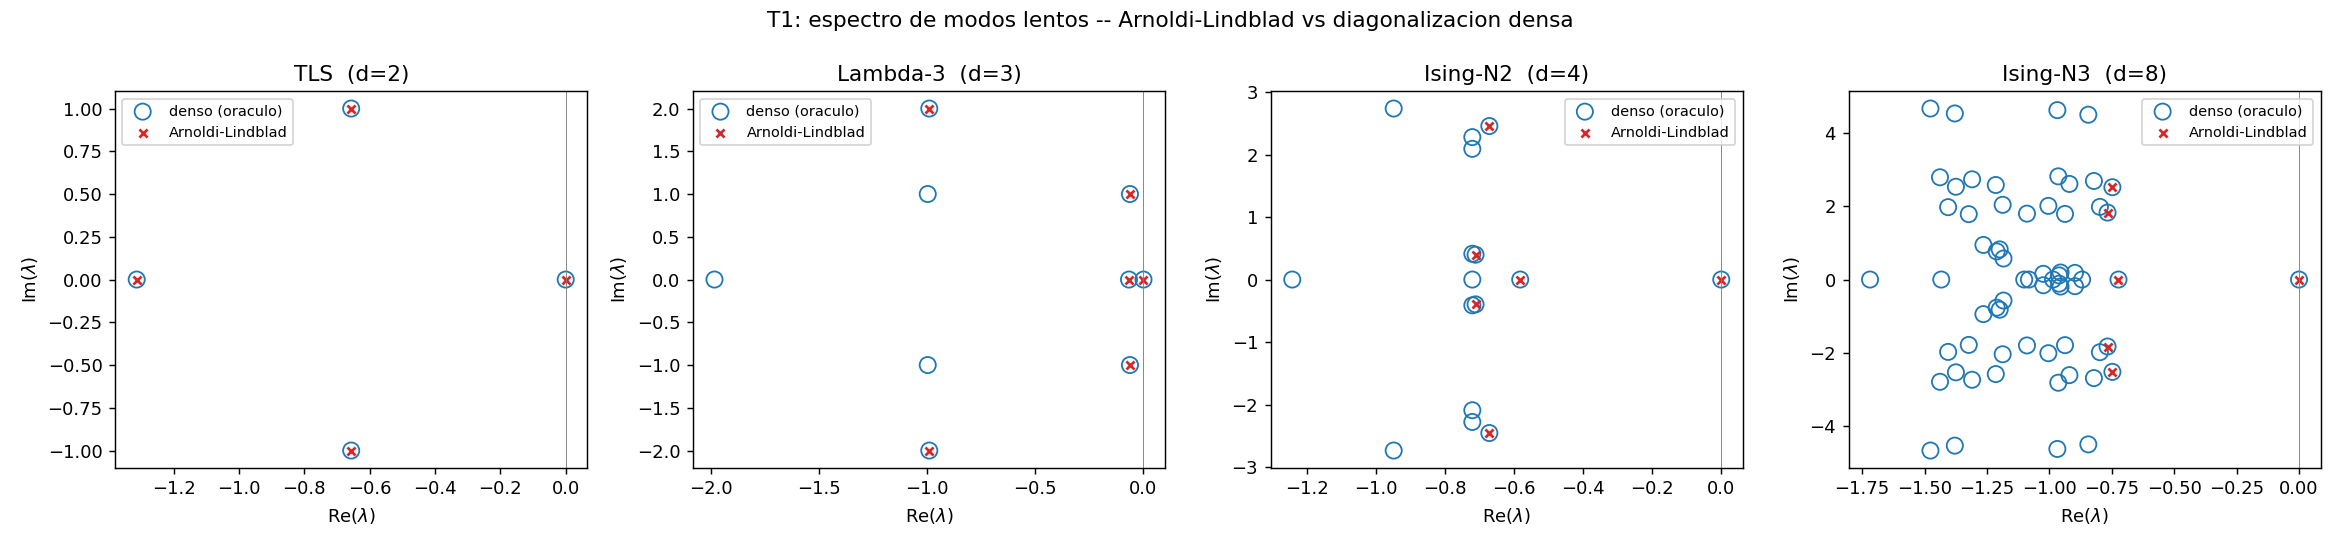
\includegraphics[width=\textwidth]{figures/t1_eigs.png}
\caption{Espectro de modos lentos: Arnoldi--Lindblad (cruces) frente a la
diagonalización densa (círculos) en el plano complejo, para los cuatro modelos.}
\label{fig:t1eigs}
\end{figure}

\subsection{Escalado paralelo}

La \cref{fig:t1scaling} y la \cref{tab:t1scaling} muestran el escalado del núcleo
C++ sobre Ising $N=7$ ($d=128$, $\dim\Lop=16\,384$). Tanto OpenMP como MPI escalan
de forma similar hasta $\sim 2.9\times$ con 4 \emph{workers}, con saturación a 8
por el ancho de banda de memoria (el \texttt{matmul} es \emph{memory-bound}). Es
notable que MPI escale prácticamente igual que OpenMP pese a la comunicación
\texttt{Allgatherv}: el cómputo $\mathcal{O}(d^3)$ amortiza el intercambio de
$\mathcal{O}(d^2)$ por \texttt{matmul}.

\begin{table}[h]
\centering
\caption{T1: speedup del SpMV distribuido (Ising $N=7$, $d=128$).}
\label{tab:t1scaling}
\begin{tabular}{cccc}
\toprule
workers & OpenMP & MPI \\
\midrule
2 & $1.79\times$ & $1.81\times$ \\
4 & $2.89\times$ & $2.71\times$ \\
8 & $2.95\times$ & --- \\
\bottomrule
\end{tabular}
\end{table}

\begin{figure}[t]
\centering
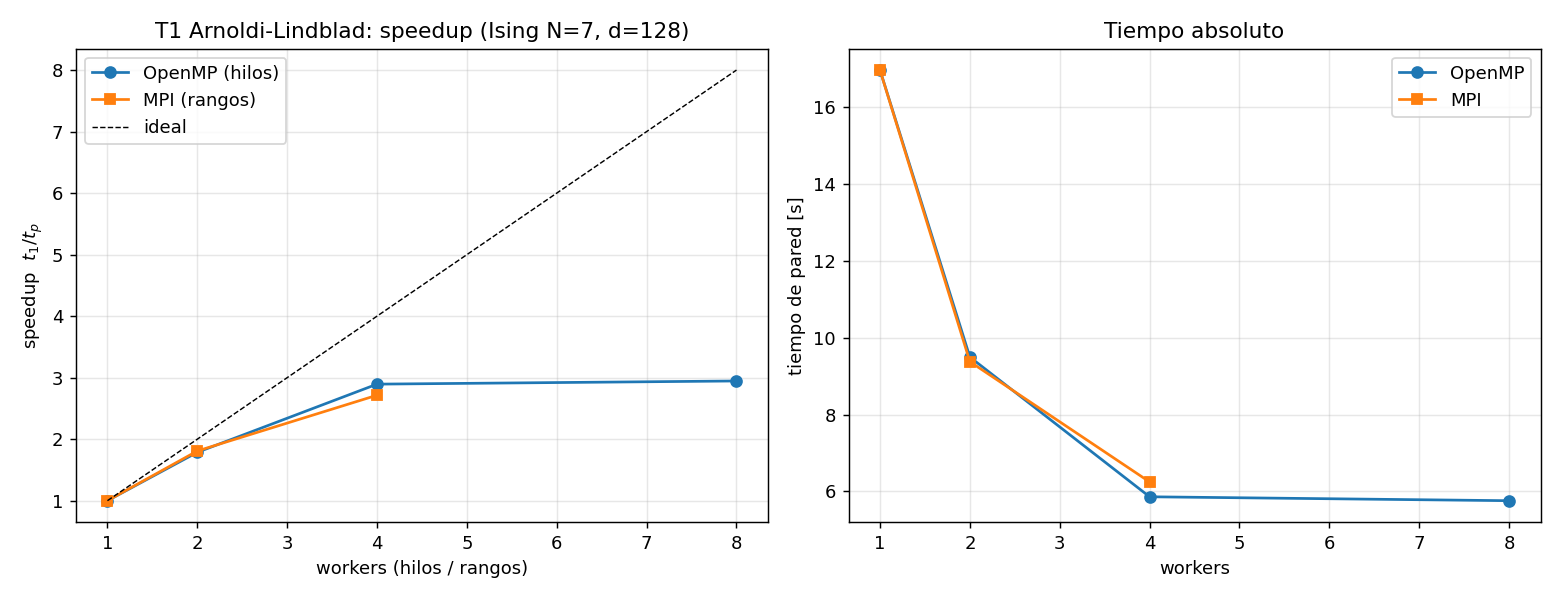
\includegraphics[width=\textwidth]{figures/t1_scaling.png}
\caption{Escalado de T1 (Arnoldi--Lindblad, Ising $N=7$): speedup y tiempo de
pared frente al número de hilos (OpenMP) y rangos (MPI).}
\label{fig:t1scaling}
\end{figure}

\medskip
\noindent\textbf{Limitación y trabajo futuro.} La distribución MPI reparte el
\emph{cómputo} del \texttt{matmul} pero mantiene los operadores replicados (la
memoria no se distribuye). El escalado real a muchos cuerpos requiere
almacenamiento disperso (CSR) de $H$ y $L_\mu$, que aprovecha que el SpMV preserva
la dispersión ($\mathcal{O}(d^2\,\mathrm{poly}\,N)$ no nulos) ---la costura de
paralelización señalada en el informe.

\chapter{T3a --- Muchos cuerpos: trayectorias cuánticas}
\label{ch:t3a}

\ideacentral{T3a valida que la \emph{dinámica de relajación} de muchos cuerpos
---el escenario donde el QMpE es físicamente rico y el Liouvilliano explícito de
T1 es imposible--- se puede simular con trayectorias estocásticas (memoria $2^N$
en vez de $4^N$), reproduciendo la ecuación maestra exacta dentro del error
estadístico $M^{-1/2}$ y con escalado \emph{casi ideal}. Es decir: la simulación
sobre la que se observaría y explotaría el efecto es correcta y escalable a
tamaños inaccesibles a T1.}

\section{Marco teórico}

Cuando $4^N$ excede la memoria disponible, el Liouvilliano explícito deja de ser
viable. El método de \textbf{trayectorias cuánticas} (Monte Carlo wavefunction;
Dalibard--Castin--Mølmer; ver Daley, \emph{Adv. Phys.} \textbf{63}, 77, 2014)
reemplaza la propagación del operador densidad $\rho\in\mathbb{C}^{d\times d}$ por
la de $M$ \emph{vectores de estado} estocásticos $\ket{\psi}\in\mathbb{C}^d$, y
recupera
\begin{equation}
    \rho_t = \mathbb{E}\big[\ket{\psi_t}\!\bra{\psi_t}\big]
           \approx \frac{1}{M}\sum_{m=1}^{M}\ket{\psi_t^{(m)}}\!\bra{\psi_t^{(m)}}.
\end{equation}
La memoria pasa de $d^2=4^N$ a $d=2^N$, lo que permite alcanzar $N$ inviables para
la ecuación maestra. El error estadístico del promedio decae como $M^{-1/2}$.

\section{Método numérico: saltos cuánticos}

Cada trayectoria evoluciona con el Hamiltoniano efectivo no hermítico
$H_{\mathrm{eff}} = H - \tfrac{i}{2}\sum_\mu L_\mu^\dagger L_\mu$. En cada paso $dt$:
\begin{align}
    \ket{\psi'} &= \ket{\psi} - i\,dt\,H_{\mathrm{eff}}\ket{\psi},
    & \delta p &= 1 - \langle\psi'|\psi'\rangle.
\end{align}
Se extrae $r\sim U[0,1]$: si $r<\delta p$ ocurre un \emph{salto}, se elige el canal
$\mu$ con probabilidad $\propto\langle\psi|L_\mu^\dagger L_\mu|\psi\rangle$ y se
aplica $\ket{\psi}\to L_\mu\ket{\psi}/\|L_\mu\ket{\psi}\|$; si no, se normaliza la
propagación determinista $\ket{\psi}\to\ket{\psi'}/\|\psi'\|$.

\paragraph{Acción matrix-free para muchos cuerpos.}
En el núcleo C++ (\texttt{T3/T3a\_trajectories/cpp/qtraj\_mpi.cpp}) ni $H$ ni los
$L_\mu$ se almacenan: la acción sobre $\ket{\psi}$ se calcula localmente,
explotando la estructura de la cadena de Ising \cref{eq:ising}. La parte diagonal
($-J\sum Z_iZ_{i+1}$ y $\sum_\mu L_\mu^\dagger L_\mu$) es un signo por estado de la
base; la parte $-h\sum_i X_i$ conecta cada estado con sus $N$ vecinos por
volteo de un bit; los saltos $\sigma_\pm^i$ son operaciones locales. El coste por
paso es $\mathcal{O}(N\,d)$, sin matrices.

\section{Implementación serial}

La referencia serial (\texttt{python/qtraj.py}, función \texttt{evolve\_serial})
promedia $M$ trayectorias en un solo proceso. Cada trayectoria usa un generador
de números aleatorios con semilla propia, garantizando independencia y
reproducibilidad.

\section{Justificación de la paralelización}

Las trayectorias son \emph{independientes}: este es el caso \emph{embarrassingly
parallel} por excelencia. La única comunicación es la reducción final del
observable promediado. Se explotan dos niveles:
\begin{itemize}
  \item \textbf{MPI} (internodo): cada rango simula $M/K$ trayectorias y el
  resultado se combina con \texttt{MPI\_Reduce}.
  \item \textbf{OpenMP} (intranodo): dentro de cada rango, las trayectorias
  locales se reparten entre hilos, cada uno con su acumulador y su RNG.
\end{itemize}
En Python, la versión \texttt{evolve\_parallel} usa \texttt{multiprocessing} como
equivalente de memoria compartida. Al no haber acoplamiento secuencial (a
diferencia de T1), se espera escalado casi ideal.

\section{Comparación y resultados}

\subsection{Convergencia y validación}

La \cref{fig:t3aconv} valida el método contra la ecuación maestra exacta (TLS): el
error RMS del promedio decae con pendiente log--log $-0.488$, en excelente acuerdo
con la ley teórica $M^{-1/2}$. La validación cruzada del núcleo C++ contra el
oráculo denso (Ising $N=3$, $M=20\,000$) da un error máximo de $8\times10^{-3}$,
dentro del error estadístico esperado.

\begin{figure}[t]
\centering
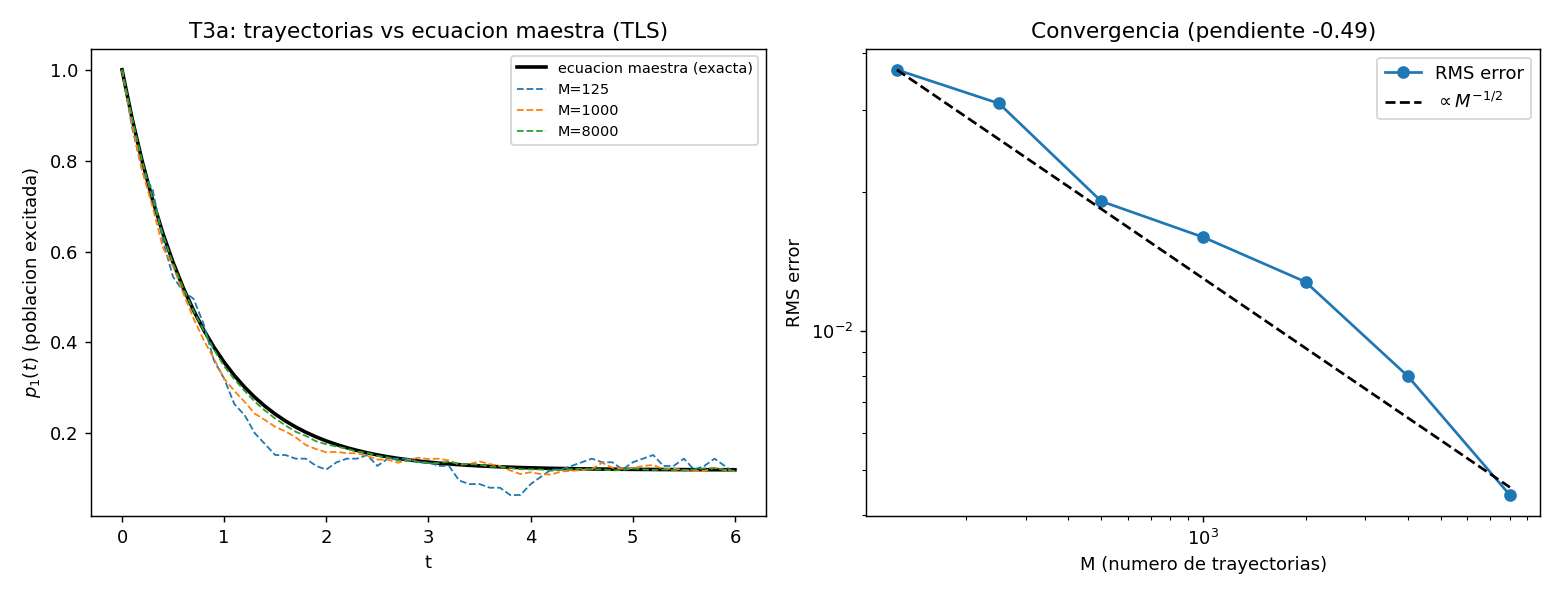
\includegraphics[width=\textwidth]{figures/t3a_convergence.png}
\caption{T3a: (izq.) población excitada del TLS, trayectorias frente a la ecuación
maestra exacta; (der.) error RMS frente a $M$, con pendiente $-0.488\approx-1/2$.}
\label{fig:t3aconv}
\end{figure}

\subsection{Escalado paralelo}

La \cref{tab:t3ascaling} y la \cref{fig:t3ascaling} muestran el escalado del núcleo
C++ sobre Ising $N=10$ ($d=1024$; el Liouvilliano denso sería $4^{10}\approx10^6$
de dimensión, imposible). El escalado es \emph{casi ideal} y prácticamente idéntico
para OpenMP y MPI, como corresponde a un problema embarrassingly parallel. El
contraste con T1 (\cref{tab:t1scaling}) es la lección central de Sistemas
Distribuidos: la estructura del acoplamiento del algoritmo determina su
escalabilidad.

\begin{table}[h]
\centering
\caption{T3a: speedup de las trayectorias distribuidas (Ising $N=10$, $d=1024$,
$M=1024$).}
\label{tab:t3ascaling}
\begin{tabular}{ccc}
\toprule
workers & OpenMP & MPI \\
\midrule
2 & $1.95\times$ & $1.96\times$ \\
4 & $3.72\times$ & $3.73\times$ \\
8 & $4.77\times$ & $4.64\times$ \\
\bottomrule
\end{tabular}
\end{table}

\begin{figure}[t]
\centering
\begin{subfigure}{0.49\textwidth}
  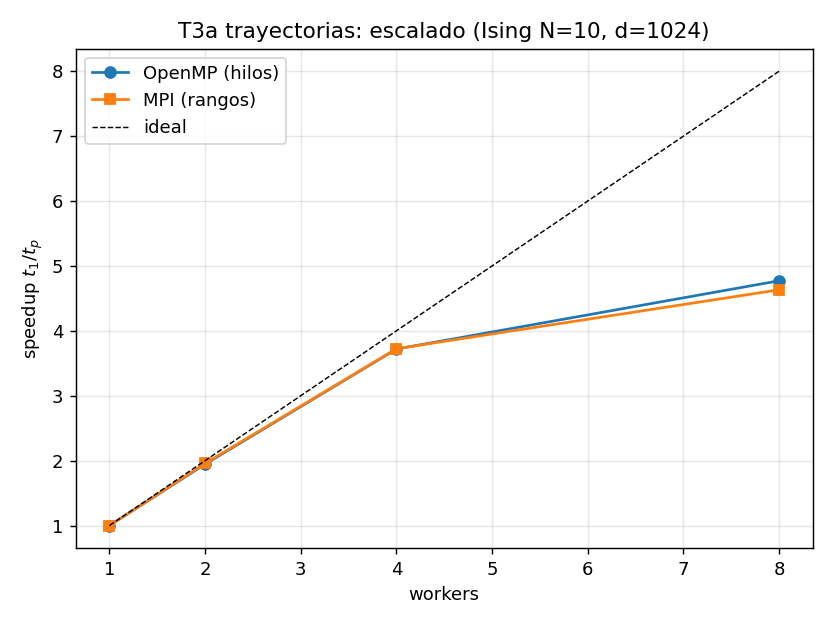
\includegraphics[width=\textwidth]{figures/t3a_scaling.png}
\end{subfigure}\hfill
\begin{subfigure}{0.49\textwidth}
  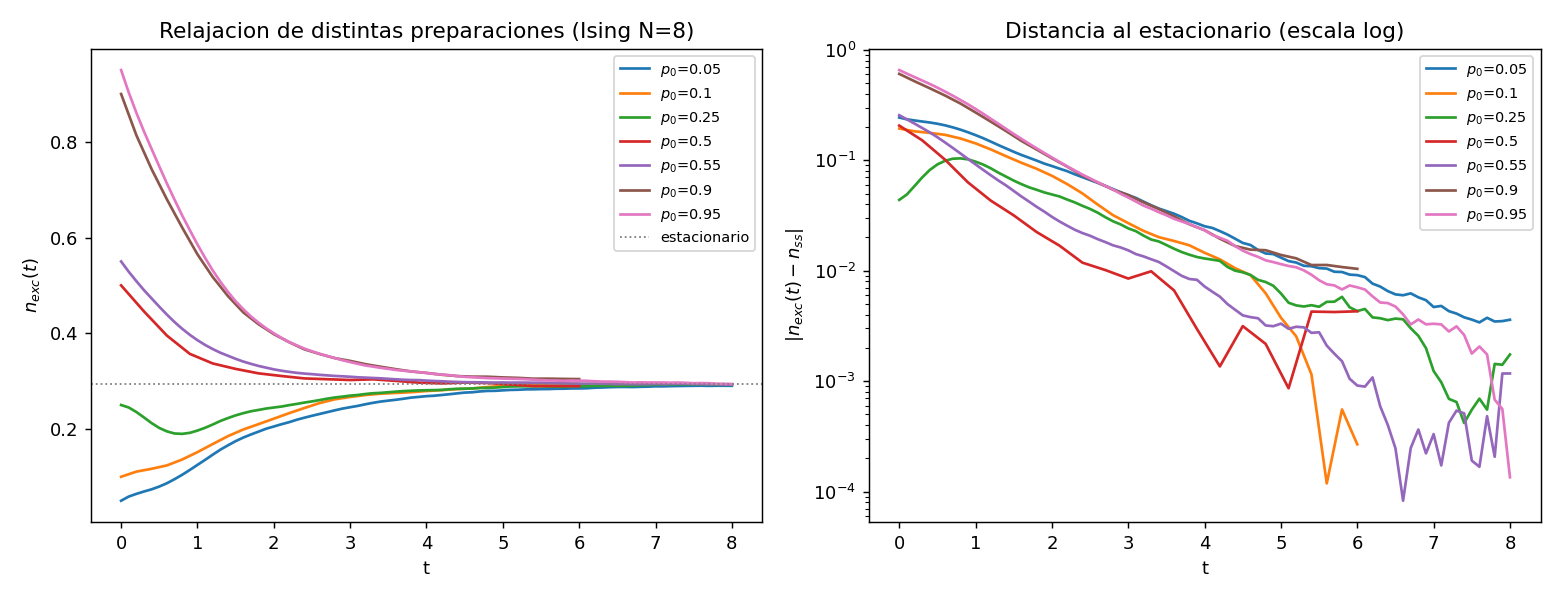
\includegraphics[width=\textwidth]{figures/t3a_curves.png}
\end{subfigure}
\caption{T3a: (izq.) escalado casi ideal de OpenMP y MPI; (der.) relajación de la
densidad de excitación de distintas preparaciones $p_0$ de la cadena de Ising
$N=8$ hacia un estado estacionario común.}
\label{fig:t3ascaling}
\end{figure}

Además, en Python el promedio con \texttt{multiprocessing} sobre el TLS alcanza un
speedup de $4.6\times$ (M=4000) frente al serial, confirmando el mismo patrón en
memoria compartida.

\chapter{T3b --- Muchos cuerpos: redes tensoriales}
\label{ch:t3b}

\ideacentral{T3b valida la vía \emph{complementaria} a muchos cuerpos: la misma
dinámica de relajación se captura con redes tensoriales (superket MPS) a coste
polinómico en la dimensión de enlace $\chi$, volviéndose \emph{exacta} al crecer
$\chi$ (error $\to10^{-7}$) y alcanzando $N=32$ ($4^{32}\approx10^{19}$, imposible
en denso). El parámetro $\chi$ ofrece un control sistemático de la precisión del
que las trayectorias (T3a) carecen.}

\section{Marco teórico}

La segunda vía para muchos cuerpos representa el operador densidad como una
\textbf{red tensorial}. En la representación vectorizada (Zwolak \& Vidal,
\emph{PRL} \textbf{93}, 207205, 2004), $\rho$ se escribe como un \emph{superket}
$\ket{\rho}\rangle$ que es un \emph{Matrix Product State} (MPS) con dimensión
física $4$ por sitio: el índice doblado $p=a\cdot2+b$ combina la fila $a$ y la
columna $b$ de cada qubit. La ecuación maestra se convierte en
\begin{equation}
    \frac{\dd}{\dd t}\ket{\rho}\rangle = \Lop\,\ket{\rho}\rangle,
\end{equation}
con $\Lop$ un operador local (suma de términos de $1$ y $2$ sitios). El coste de
representar y evolucionar el MPS es polinómico en la \emph{dimensión de enlace}
$\chi$, que controla el entrelazamiento (de operador) capturado. Si $\chi$ se
mantiene acotado, se alcanzan tamaños $N$ inaccesibles a cualquier método exacto.

\section{Método numérico: TEBD disipativo}

Se usa \textbf{TEBD} (Time-Evolving Block Decimation). El Liouvilliano se
descompone en generadores de \emph{bond} $\Lop=\sum_b \Lop_b$, asignando cada
término de un sitio a un bond adyacente para evitar doble conteo. La evolución
$e^{dt\Lop}$ se trotteriza con el esquema de Strang de segundo orden,
\begin{equation}
    e^{dt\Lop}\approx
    \Big(\!\!\prod_{b\,\text{par}}\! e^{\frac{dt}{2}\Lop_b}\Big)
    \Big(\!\!\prod_{b\,\text{impar}}\! e^{dt\Lop_b}\Big)
    \Big(\!\!\prod_{b\,\text{par}}\! e^{\frac{dt}{2}\Lop_b}\Big),
\end{equation}
donde cada compuerta $e^{dt\Lop_b}$ actúa sobre dos sitios contiguos del superket.
Tras aplicar una compuerta, el tensor conjunto se reseparaa por SVD y se
\emph{trunca} a los $\chi$ mayores valores singulares. Los generadores locales se
construyen reutilizando \texttt{common.qmpe.build\_liouvillian} (en base
\emph{column-stacking}) y permutando los índices al orden site-local $p=a\cdot2+b$;
la exponencial $e^{dt\Lop_b}$ se calcula por descomposición espectral de la matriz
$16\times16$. Los observables ($\Tr\rho$, densidad de excitación) se obtienen
contrayendo el MPS con los covectores $\langle\!\langle\mathbb{1}|$ y
$\langle\!\langle n_k|$.

\section{Implementación serial}

El núcleo serial está en \texttt{T3/T3b\_tensor\_networks/python/mpdo\_tebd.py}: la
clase \texttt{SuperketMPS} (tensores $(D_l,4,D_r)$) implementa la aplicación de
compuertas con truncación SVD, la traza y los valores esperados. La función
\texttt{evolve\_tebd} realiza la evolución de Strang completa.

\section{Justificación de la paralelización}

El paralelismo de TEBD es \emph{estructurado}: dentro de una capa de Trotter, las
compuertas sobre bonds \emph{disjuntos} ---los pares $(0,1),(2,3),\dots$ o los
impares $(1,2),(3,4),\dots$--- no comparten tensores y pueden aplicarse
simultáneamente. Cada compuerta realiza una SVD de coste $\mathcal{O}(\chi^3)$.
Como numpy libera el GIL durante la SVD/BLAS, se paralelizan con \emph{hilos}
(\texttt{ThreadPoolExecutor}) sin coste de serialización ---a diferencia de
\texttt{multiprocessing}, que requeriría copiar los tensores. Este patrón es
intermedio entre el SpMV acoplado de T1 y las trayectorias independientes de T3a.

\paragraph{Mapeo a memoria distribuida.} Para muchos nodos, el esquema se mapea a
MPI repartiendo segmentos contiguos de la cadena entre rangos, con intercambio de
los tensores de frontera por capa de Trotter; queda como trabajo futuro.

\section{Comparación y resultados}

\subsection{Validación y convergencia en $\chi$}

La \cref{fig:t3bval} valida el TEBD contra la ecuación maestra exacta (Ising
$N=4$): el error decae sistemáticamente al aumentar $\chi$,
\[
  6\times10^{-2}\ (\chi{=}1)\;\to\; 3\times10^{-3}\ (\chi{=}4)\;\to\;
  6.3\times10^{-7}\ (\chi{=}16),
\]
alcanzando precisión esencialmente exacta cuando $\chi$ iguala el rango máximo del
sistema ($\chi=16$ para $N=4$). Esto confirma la correctitud del esquema de
índices y de la truncación.

\begin{figure}[t]
\centering
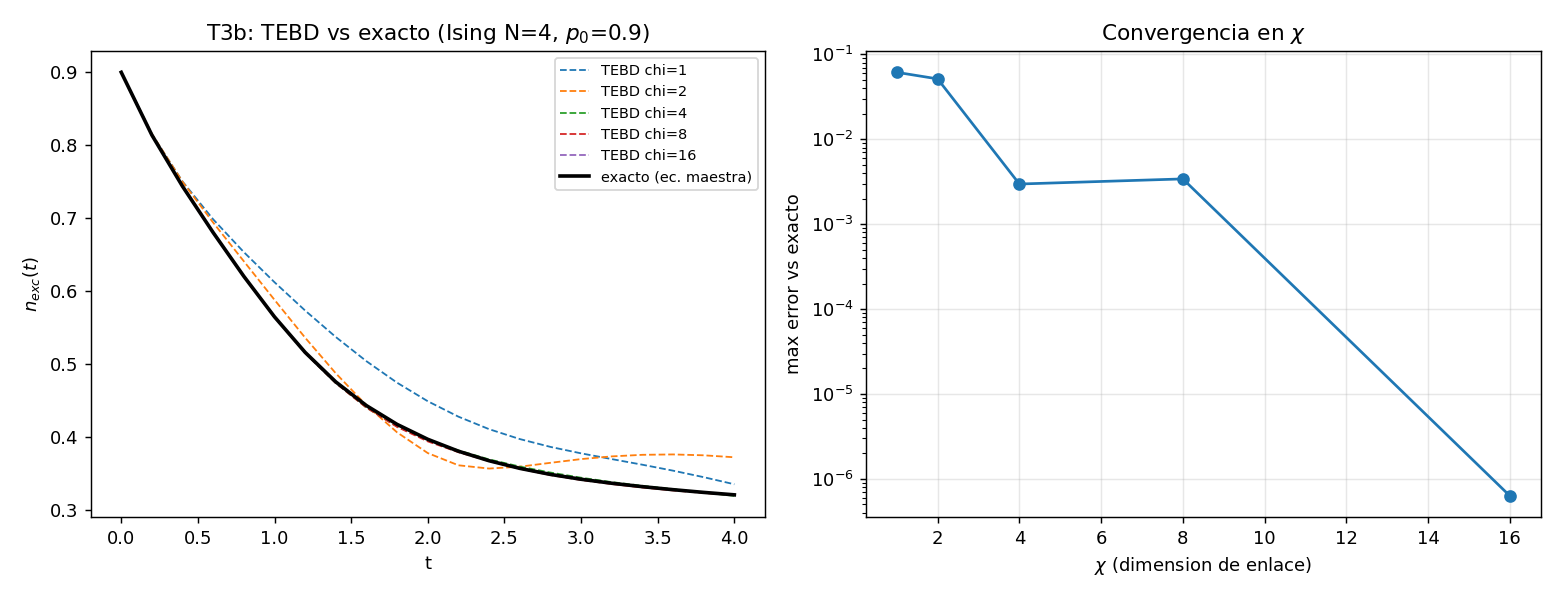
\includegraphics[width=\textwidth]{figures/t3b_validation.png}
\caption{T3b: (izq.) densidad de excitación, TEBD a distintos $\chi$ frente al
exacto (Ising $N=4$); (der.) error máximo frente a $\chi$ (escala log).}
\label{fig:t3bval}
\end{figure}

\subsection{Escalado y muchos cuerpos}

La \cref{fig:t3bscaling} muestra el escalado del TEBD paralelo por compuertas
(Ising $N=20$, $\chi=48$, con BLAS de un hilo para aislar el paralelismo): $1.84\times$
(2 hilos), $2.72\times$ (4) y $3.61\times$ (8). El escalado es bueno pero no ideal:
el número de bonds disjuntos por capa ($\sim N/2$) y el desbalance de carga (los
tensores centrales alcanzan mayor $\chi$ que los de los extremos) limitan la
eficiencia, ilustrando el paralelismo estructurado con granularidad media.

\begin{table}[h]
\centering
\caption{T3b: speedup del TEBD paralelo por compuertas (Ising $N=20$, $\chi=48$).}
\label{tab:t3bscaling}
\begin{tabular}{cc}
\toprule
hilos & speedup \\
\midrule
2 & $1.84\times$ \\
4 & $2.72\times$ \\
8 & $3.61\times$ \\
\bottomrule
\end{tabular}
\end{table}

\begin{figure}[t]
\centering
\begin{subfigure}{0.49\textwidth}
  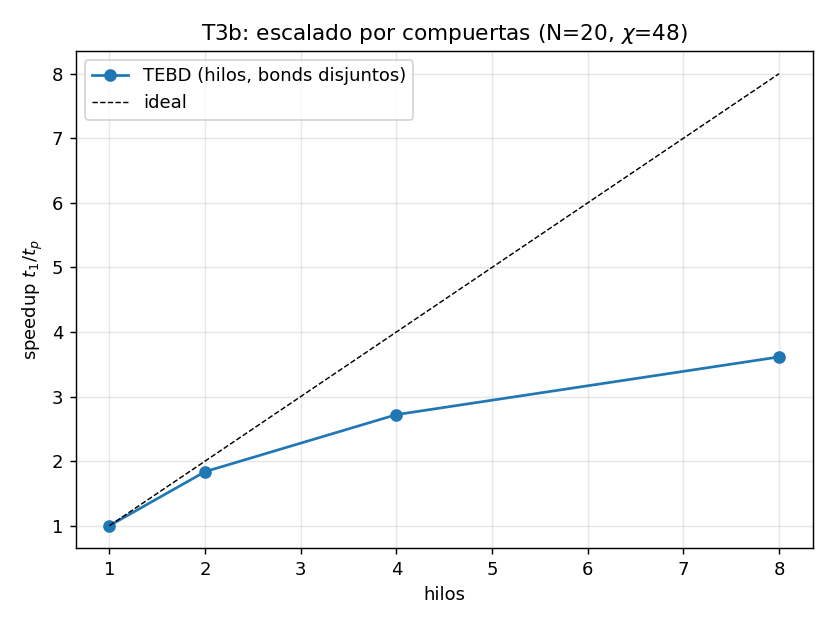
\includegraphics[width=\textwidth]{figures/t3b_scaling.png}
\end{subfigure}\hfill
\begin{subfigure}{0.49\textwidth}
  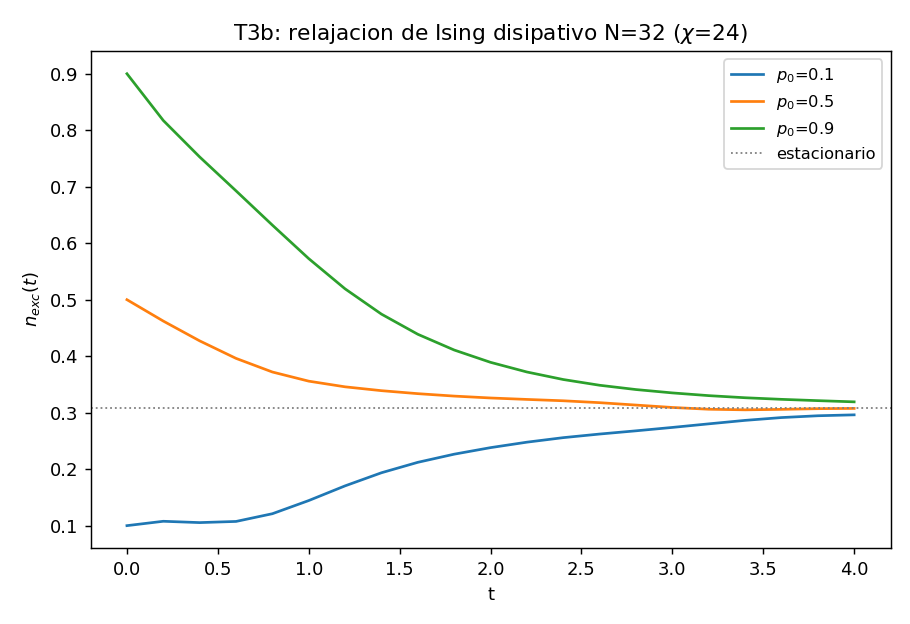
\includegraphics[width=\textwidth]{figures/t3b_largeN.png}
\end{subfigure}
\caption{T3b: (izq.) escalado por compuertas (N=20, $\chi=48$); (der.) relajación
de la cadena de Ising disipativa con $N=32$ sitios ($4^{32}\approx1.8\times10^{19}$,
imposible en denso), evolucionada con $\chi=24$ en $\sim3.6$\,s.}
\label{fig:t3bscaling}
\end{figure}

La demostración de muchos cuerpos evoluciona $N=32$ sitios ---cuyo Liouvilliano
denso tendría dimensión $4^{32}\approx1.8\times10^{19}$, absolutamente
inalcanzable--- con $\chi=24$ en unos $3.6$\,s por preparación. Las tres
preparaciones ($p_0=0.1,0.5,0.9$) relajan hacia un estacionario común, mostrando
que la red tensorial captura la dinámica de relajación con recursos polinómicos.

\chapter{Conclusiones generales}
\label{ch:conclusiones}

Este trabajo implementó y validó las tareas computacionales \textbf{T1} y
\textbf{T3} del estudio numérico del efecto Mpemba cuántico, cada una en versión
serial y paralela, sobre la cadena de Ising transversa disipativa.

\ideacentral{La tesis (\cref{sec:tesis}) se cumple: el QMpE es geometría espectral
de un generador no normal, así que verificarlo y explotarlo en HPC equivale a
\emph{calcular} su estructura y dinámica de relajación de forma correcta y
escalable. T1 entrega el \textbf{diagnóstico que predice} el efecto (modos lentos,
$a_k$); T3a/T3b entregan la \textbf{simulación} de la relajación en muchos cuerpos.
Los datos confirman las dos exigencias: \emph{correctitud} (todas validadas contra
el oráculo exacto) y \emph{escalabilidad} (la habilitación para explotar).}

\section*{Correctitud}

Los tres métodos se validaron contra un mismo oráculo exacto (diagonalización e
integración densa del Liouvilliano, $N\lesssim4$):
\begin{itemize}
  \item \textbf{T1} (Arnoldi--Lindblad) reproduce los autovalores lentos con error
  $10^{-13}$--$10^{-5}$ y el estado estacionario a $10^{-11}$.
  \item \textbf{T3a} (trayectorias) converge con la ley estadística $M^{-1/2}$
  (pendiente medida $-0.488$) y coincide con la ecuación maestra a $8\times10^{-3}$
  con $M=2\times10^4$.
  \item \textbf{T3b} (TEBD) converge a la solución exacta al aumentar $\chi$,
  alcanzando $6\times10^{-7}$ cuando $\chi$ iguala el rango del sistema.
\end{itemize}

\section*{La lección de Sistemas Distribuidos: la estructura del acoplamiento
determina la escalabilidad}

El resultado más instructivo es el \emph{contraste} entre los tres patrones de
paralelismo, resumido en la \cref{tab:resumen}:

\begin{table}[h]
\centering
\caption{Comparación de los tres patrones de paralelismo (speedup a 4 workers).}
\label{tab:resumen}
\begin{tabular}{lll c}
\toprule
Tarea & Patrón de paralelismo & Tecnología & speedup (4) \\
\midrule
T1  & SpMV \emph{secuencialmente acoplado} & MPI+OpenMP (datos) & $\sim2.8\times$ \\
T3a & trayectorias \emph{independientes}   & MPI+OpenMP (tareas) & $\sim3.7\times$ \\
T3b & compuertas \emph{disjuntas} por capa & hilos (estructurado) & $\sim2.7\times$ \\
\bottomrule
\end{tabular}
\end{table}

\begin{itemize}
  \item \textbf{T1} está limitado porque Arnoldi es secuencialmente acoplado: solo
  el SpMV interno paraleliza, y su naturaleza \emph{memory-bound} satura el
  escalado en el hardware de prueba. La comunicación \texttt{Allgatherv} de MPI se
  amortiza por el cómputo $\mathcal{O}(d^3)$, de modo que MPI iguala a OpenMP.
  \item \textbf{T3a} es \emph{embarrassingly parallel} y escala casi idealmente,
  con OpenMP y MPI indistinguibles; es el mejor candidato a escalar a muchos nodos.
  \item \textbf{T3b} tiene paralelismo estructurado de granularidad media,
  limitado por el número de bonds disjuntos y el desbalance de carga (los tensores
  centrales soportan mayor $\chi$).
\end{itemize}

\section*{Alcance en muchos cuerpos}

Las tareas T3 cumplen su promesa de superar la barrera $4^N$: T3a simula $N=10$
($d=1024$) con trayectorias de memoria $2^N$, y T3b alcanza $N=32$
($4^{32}\approx1.8\times10^{19}$) con dimensión de enlace acotada $\chi=24$. Ambas
son inalcanzables para la representación explícita del Liouvilliano que requiere T1.

\section*{Trabajo futuro}

Las costuras de paralelización pendientes, en línea con el informe base, son:
(i) almacenamiento disperso (CSR) de $H$ y $L_\mu$ para distribuir realmente la
\emph{memoria} en T1 (no solo el cómputo); (ii) trayectorias en GPU para T3a;
(iii) TEBD distribuido por segmentos de cadena con frontera MPI para T3b; y (iv)
combinar T1 y T3b (espectro del Liouvilliano con redes tensoriales) para el gap en
cadenas largas. En conjunto, las tres tareas forman una cadena de herramientas
coherente: T1 diagnostica el efecto en pocos cuerpos, y T3a/T3b lo exploran en el
régimen de muchos cuerpos donde el fenómeno es físicamente más rico.


\end{document}
